\chapter{Reflection}

What happens when light hits a mass?

In a previous chapter, we talked about light as a wave, and we
mentioned that each color in the rainbow is a different
wavelength. You can also think of light as particles of energy called
\newterm{photons}. And every photon comes with an amount of energy
that determines what color it is.

When we are talking about light interacting with objects, your
intuition will be right more often if you think of light as a beam of
photons.

When a photon comes from the sun and hits an object, one of several
things can happen:

\begin{itemize}
  
  \item The energy of the photon is absorbed by the object. It makes the
    object a little warmer. If a large proportion of photons hitting the
    mass are absorbed like this, we say the object is ``black''.\index{absorption!photon}

 \item The photon bounces off the object.  If the surface is very
   smooth, the photons bounce in a predictable manner, and we call
   this \newterm{reflection} and we say the object is ``shiny''.\index{reflection}

 \item If the surface is rough and the photons are not absorbed, the
   photons are scattered in random directions.  We call this
   \newterm{diffusion}.  If most of the photons hitting an object are
   bounced in random directions, we say that the object is ``white''.\index{diffusion}

 \item The photon passes through the mass.  If the mass has smooth
   surfaces and a consistent composition, the photons will pass throught the
   mass in a predictable manner.  We say that the mass is ``transparent''.\index{transparent}

 \item If the photons pass through, but in an unpredictable,
   scattering manner, we say the mass is ``translucent''. \index{translucent}

\end{itemize}

No object absorbs every photon, but chemists are always coming up with
``blacker'' materials. Vantablack, for example, is a super-black paint
that absorbs 99.965\% of all photons in the visible spectrum.\index{Vantablack}

No object reflects every photon, but a mirror is pretty close. Let's
talk about reflections in a mirror.\index{mirror}

\section{Reflection}

When a beam of light hits mirror, it bounces of the mirror at the same
angle it approached from.  That is, if it approaches nearly
perpendicular to the mirror, it departs nearly perpendicular to the
mirror.  If it hits the mirror at a glancing angle, it departs at an
angle close to the mirrors surface.

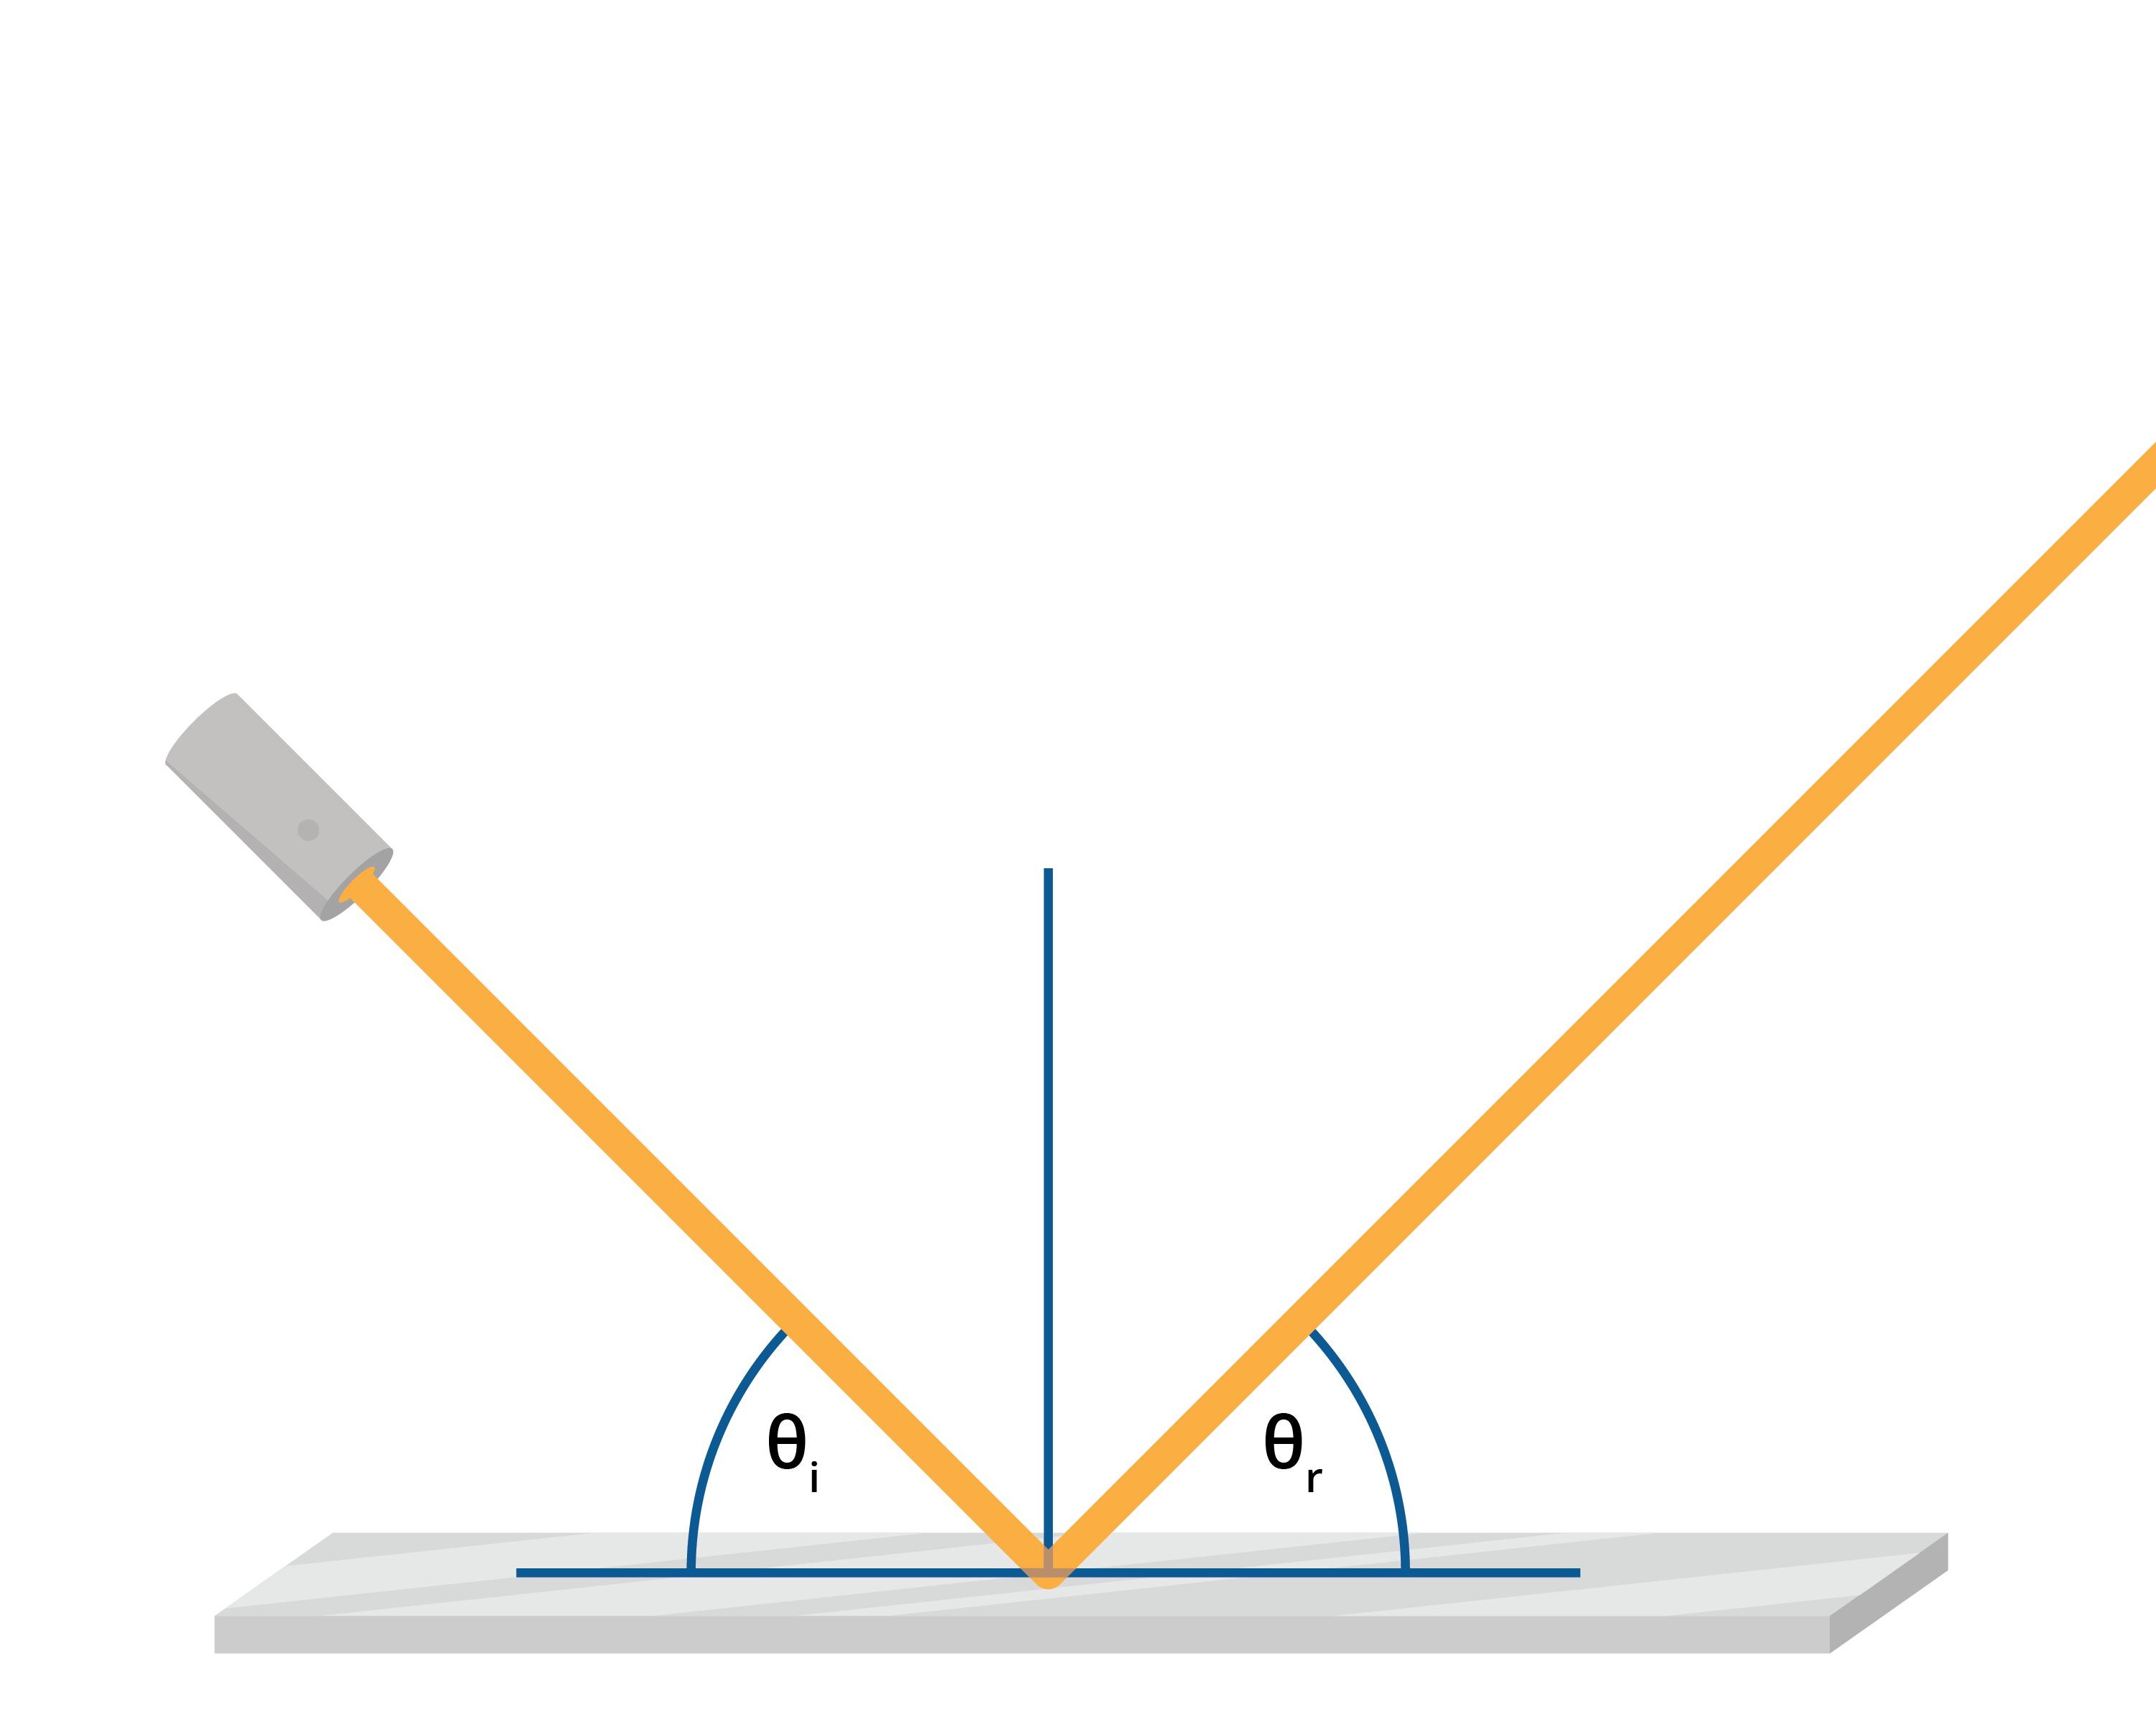
\includegraphics[width=1\textwidth]{reflection.png}

\begin{mdframed}[style=important, frametitle={Law of Reflection}]

The angle of incidence, denoted as $\theta_i$, is equal to
the angle of reflection, denoted as $\theta_r$. This law can be
mathematically expressed as:\index{reflection!law of}

$$\theta_i = \theta_r$$
 
where $\theta_i$ is the angle between the incident light ray and the
normal to the surface, and $\theta_r$ is the angle between the
reflected light ray and the normal.

\begin{tikzpicture}[scale=5]
  \draw [black,thick](-0.7,0)--(0.7,0) node [midway, anchor=north]{Mirror};
  \draw [sdkblue,dashed,->] (0,0) -- (0,0.7) node [anchor=south]{Normal};
  \draw [sdkblue] (0,0.08) -- (0.08, 0.08) -- (0.08, 0);
  \draw [->](-0.5,0.8)--(-0.04,0.05);
  \draw [->](0,0)--(0.5,0.8);
  \draw [sdkblue,<->] (0, 0.3) arc (90:122:0.3)
  node [midway, anchor=south] {$\theta_i$};  
  \draw [sdkblue,<->] (0, 0.3) arc (90:58:0.3)
  node [midway, anchor=south] {$\theta_r$};
\end{tikzpicture}

\end{mdframed}

\begin{Exercise}[title={Law of Reflection}, label=law_of_reflection]

  You are standing 4 meters from a mirror hung on a wall.  The bottom
  of the mirror is the same height as your chin, so you can't see your
  whole body.  You stick a piece of masking tape to your body.

  You walk forward until you are only 3 meters from the mirror, and
  put a piece of masking tape on your body at the new cut-off point.  Is the new
  masking tape higher or lower on your body?
  
\end{Exercise}
\begin{Answer}[ref=law_of_reflection]

 Assuming the mirror is truly vertical and the floor is truly
 horizontal, the new cut off should be exactly the same as the old
 one: It should be below your chin the same amount that your eyes are
 above your chin.

 \textit{Illustration Here}

\end{Answer}

\begin{Exercise}[title={Photons and Color}, label=photon_color]

  There are red photons.

  Are there black photons?

  Are there white photons?

  Are there yellow photons?
  
\end{Exercise}
\begin{Answer}
  
\textit{Are there white photons?}  No. What we call ``white'' is a
blend of photons that are several different colors.

Some people like to say white light is the combination of all visible
colors of photons in equal amounts. That seems oddly specific and unusual.

Maybe it is better to imagine it from the human experience of white
light. In our eyes, we have three different types of color-sensing
cones, which generally correspond to the the red, the green, and the
blue regions of the spectrum.  When all three are excited about equal
amounts, humans experience that as white.  On your computer screen,
for example, what you see as white is just a blend of three colors of
photons: a red, a green, and a blue.

\textit{Are there black photons?}  No. What we call ``black'' is an
absence of photons in the visible range.

\textit{Are there yellow photons?} Yes! There is a region of the color
spectrum that is yellow. It has a wavelength of about 527 nm.  Photons
at this energy level excite both our green-sensitive and red-sensitive
cones.
Your computer monitor does not actually create light with a 527 nm
wavelength. Instead, it creates red light and green light, which our
eyes interpret as yellow.

\end{Answer}

\section{Curved Mirrors}

Flat mirrors are common and useful, but things get more interesting
once you bend the mirrors. In this section, we are going to talk about
a few different kinds of curved mirrors.\index{circle!reflections in}

\subsection{The Reflective Properties of Circles and Spheres}

For example, if you were inside a circular room (a cylinder,
actually), you could imagine standing in the center and pointing a
flash light in any horizontal direction.  The beam of light would
bounce right back to you.

\begin{tikzpicture}[scale=1]
  \coordinate (a) at (0,0);
  \coordinate (b) at ({3 * cos(30)}, {3 * sin(30)});
  \draw [black, thick] (a) circle (3);
  \filldraw [sdkblue] (a) circle (2pt);
  \filldraw [sdkblue] (b) circle (2pt);
  \draw [sdkblue,<->] ({0.2 * cos(30)},{0.2 * sin(30)})--({2.8 * cos(30)},{2.8 * sin(30)});
\end{tikzpicture}

How do you know this?  Because the tangent line is always perpendicular to the radius to the point of tangency:

\begin{tikzpicture}[scale=1.4]
  \coordinate (a) at (0,0);
  \coordinate (b) at ({3 * cos(30)}, {3 * sin(30)});
  \draw [black, thick] (3,0) arc (0:80:3);
  \filldraw [sdkblue] (a) circle (2pt);
  \filldraw [sdkblue] (b) circle (2pt);
  \draw [sdkblue,<->] ({0.2 * cos(30)},{0.2 * sin(30)})--({2.8 * cos(30)},{2.8 * sin(30)});
  \clip (-.1, -.1) rectangle (4,3);
  \draw [dashed] (0,{3 / sin(30)}) -- ({3 / cos(30)},0);
\end{tikzpicture}

You could create a spherical room with mirror walls. You'd
create a platform in the center where you could stand, and if you
pointed your flashlight in any direction, its beam of light would
shine back at you.

\subsection{Ellipses and Ellipsoids}

Intuitively, you know what an ellipse is: it is an oval. But the
ellipse is actually an oval with some special properties.  This is a
good time to talk about those properties.\index{ellipse}

Mathematicians talk about a \newterm{standard} ellipse. A standard ellipse is
centered on the origin $(0,0)$ and its long axis is parallel with the
$x$-axis or the $y$-axis.

\begin{mdframed}[style=important, frametitle={Equation for a Standard Ellipse}]

To be precise, a standard ellipse is the set of points $(x, y)$ that
are solutions to the equation

$$\frac{x^2}{a^2} + \frac{y^2}{b^2} = 1$$


Note that $(a,0), (-a, 0), (0, b), (0,-b)$ are all part of the
set. The complete set looks like this:

\begin{tikzpicture}[scale=2]
  \draw [sdkblue, <->] (-2.5, 0)--(2.5, 0); \draw [sdkblue, <->] (0,
  -1.5)--(0, 1.5); \draw (0,0) ellipse (2 and 1); \filldraw [sdkblue]
  (-2, 0) circle (1pt) node [anchor=east] {$-a$}; \filldraw [sdkblue]
  (2, 0) circle (1pt) node [anchor=west] {$a$}; \filldraw [sdkblue]
  (0, -1) circle (1pt) node [anchor=north] {$-b$}; \filldraw [sdkblue]
  (0, 1) circle (1pt) node [anchor=south] {$b$};
\end{tikzpicture}

The area contained inside this ellipse is given by

$$A = \pi a b$$


\end{mdframed}


We can now talk about two special points: the \newterm{foci}.  Each
focal point is on the long axis of the ellipse.  Let's assume for a
second that $a > b$.  (Everything works the same if $b > a$, but it
gets confusing if we try to deal with both cases simultaneously.)\index{ellipse!focus points}

If $p$ is a point on the ellipse, the distance from $p$ to focal point 1
plus the distance from $p$ to focal point 2 is always $2a$.

\begin{tikzpicture}[scale=2]
  \coordinate (p) at (0.7, 0.93674969975976);
  \coordinate (f1) at (-1.732050807568877, 0);
  \coordinate (f2) at (1.732050807568877, 0);
  \draw [sdkblue, <->] (-2.5, 0)--(2.5, 0);
  \draw [sdkblue, <->] (0, -1.5)--(0, 1.5);
  \draw (0,0) ellipse (2 and 1);
  \filldraw [sdkblue] (-2, 0) circle (1pt) node [anchor=east] {$-a$};
  \filldraw [sdkblue] (2, 0) circle (1pt) node [anchor=west] {$a$};
  \filldraw [sdkblue] (0, -1) circle (1pt) node [anchor=north] {$-b$};
  \filldraw [sdkblue] (0, 1) circle (1pt) node [anchor=south] {$b$};
  \filldraw (p) circle (1pt) node [anchor=south] {$p$};
  \filldraw (f1) circle (1pt) node [anchor=north] {$f_1$};
  \filldraw (f2) circle (1pt) node [anchor=north] {$f_2$};
  \draw [dashed] (f1) -- (p) node [midway, anchor=south] {$d$};
  \draw [dashed] (f2) -- (p) node [midway, anchor=north] {$2a - d$};
\end{tikzpicture}

How do we find the foci? We know they are on the long axis and that
they are symmetrical across the short axis. All we need to know is how
far are they from the short axis.

\begin{mdframed}[style=important, frametitle={Distance from Center to the Foci}]

If you have an ellipse with a long axis that extends $a$ from the center
and a short axis that extends $b$ from the center.  The foci
lie on the long axis and are $c$ from the center.  Where

$$c = \sqrt{a^2 - b^2}$$

\end{mdframed}

\begin{Exercise}[title={Foci of an ellipse}, label=ellipse_foci]
  
You need to draw an ellipse that is 12 cm long and 7 cm wide.  You
have a string, two pushpins, a ruler, and a pencil. Using the ruler,
you draw two perpendicular axes.

You will stick one pin at each focal point.  Each end of the string
will be tied to a push pin. Using the pencil to keep the string taut, you will draw
an ellipse.

\begin{tikzpicture}[scale=.2]
  \coordinate (p) at (-3, 6.77772085586298);
  \coordinate (f1) at (-9.746794344808964, 0);
  \coordinate (f2) at (9.746794344808964, 0);
  \draw [sdkblue, <-] (-14, 0)--(12, 0);
  \draw [sdkblue, <-] (0, -9)--(0, 7);
  \draw (0,0) ellipse (12 and 7);
  \filldraw [sdkblue] (-12, 0) circle (4pt);
  \filldraw [sdkblue] (12, 0) circle (4pt) node [anchor=west] {12 cm};
  \filldraw [sdkblue] (0, -7) circle (4pt);
  \filldraw [sdkblue] (0, 7) circle (4pt) node [anchor=south] {7 cm};
  \filldraw (p) circle (4pt) ;
  \filldraw (f1) circle (4pt);
  \filldraw (f2) circle (4pt);
  \draw [dashed] (f1) -- (p);
  \draw [dashed] (f2) -- (p);
\end{tikzpicture}

How far from the short axis are the pushpins placed?

How long is the string between them?

\end{Exercise}
\begin{Answer}[ref=ellipse_foci]

  The length of the string is easy: $2 \times 12 = 24$ cm.

  The distance from the center to the focal point is $\sqrt{12^2 - 7^2} approx 6.78$ cm.

  \begin{tikzpicture}[scale=.2]
  \coordinate (p) at (-3, 6.77772085586298);
  \coordinate (f1) at (-9.746794344808964, 0);
  \coordinate (f2) at (9.746794344808964, 0);
  \draw [sdkblue, <-] (-14, 0)--(12, 0);
  \draw [sdkblue, <-] (0, -9)--(0, 7);
  \draw (0,0) ellipse (12 and 7);
  \filldraw [sdkblue] (-12, 0) circle (4pt);
  \filldraw [sdkblue] (12, 0) circle (4pt) node [anchor=west] {12 cm};
  \filldraw [sdkblue] (0, -7) circle (4pt);
  \filldraw [sdkblue] (0, 7) circle (4pt) node [anchor=south] {7 cm};
  \filldraw (p) circle (4pt) ;
  \filldraw (f1) circle (4pt);
  \filldraw (f2) circle (4pt);
  \draw [dashed] (f1) -- (p) node [midway, anchor=south] {$d$};
  \draw [dashed] (f2) -- (p) node [midway, anchor=south] {$24 - d$};
  \draw (6,0) node [anchor=north] {6.78 cm};
\end{tikzpicture}

\end{Answer}

\subsubsection{The Reflective Property of Ellipses}

Here is something else that is wonderful about an ellipse: Pick any
point $p$ on the ellipse. Draw a line from $p$ to each focal point.
Draw the line tangent to the ellipse at $p$.  Fact: The angle between
the tangent and the line to focal point 1 is equal to the angle between the
tangent and the line to focal point 2.

\begin{tikzpicture}[scale=2]
  \coordinate (p) at (0.7, 0.93674969975976);
  \coordinate (f1) at (-1.732050807568877, 0);
  \coordinate (f2) at (1.732050807568877, 0);
  \clip (-2.5, -.4) rectangle (5.5,2);
  \draw [sdkblue] (-2.1, 0)--(2.1, 0);
  \draw [sdkblue] (0, -1.1)--(0, 1.1);
  \draw (0,0) ellipse (2 and 1);
  \filldraw (p) circle (1pt) node [anchor=south] {$p$};
  \filldraw (f1) circle (1pt) node [anchor=north] {$f_1$};
  \filldraw (f2) circle (1pt) node [anchor=north] {$f_2$};
  \draw [sdkblue] (f1) -- (p);
  \draw [sdkblue] (f2) -- (p);
  \coordinate (t1) at (-0.2829937278, 1.120388832);
  \coordinate (t2) at (1.682993728, 0.7531105671); 
  \draw [dashed, thick]  (t1)--(t2);
  \draw [sdkblue, <->] (t1) arc (169.4181988:201.0651201:1)
     node [midway, anchor=east] {$\theta$};
  \draw [sdkblue, <->] (t2) arc (-10.5818012:-42.22872252:1)
     node [midway, anchor=east] {$\theta$};
\end{tikzpicture}

This is known as ``The Reflective Property of Ellipses.''

Imagine you and your friend Fred are at an ellipse-shaped skating rink and
edge of the rink are mirrored.  You sit at one focal point and your friend
sits at the other, if you point a flashlight at the mirror (in any
direction!) the beam will bounce off the wall and head directly for
Fred.

If Fred ducks out of the way, the beam will bounce again and
head back to you.

\begin{tikzpicture}[scale=4]
  \coordinate (p) at (0.7, 0.93674969975976);
  \coordinate (p2) at (1.95763,-0.204758);
  \coordinate (f1) at (-1.732050807568877, 0);
  \coordinate (f2) at (1.732050807568877, 0);
  \draw (0,0) ellipse (2 and 1);
  \filldraw [sdkblue] (p) circle (0.5pt);
  \filldraw [sdkblue] (p2) circle (0.5pt);
  \filldraw (f1) circle (1pt) node [anchor=north] {You};
  \filldraw (f2) circle (1pt) node [anchor=north] {Fred};
  \draw [sdkblue, ->] (f1) -- (p);
  \draw [sdkblue, ->] (p) -- (p2);
  \draw [sdkblue, ->] (p2) -- (f1);
  \coordinate (b1) at (0.6081804337,0.4452528358);
  \coordinate (b2) at (1.219613217,0.1039995564);
  \draw [dashed] (p)--(b1);
  \draw [dashed] (p2)--(b2);
  \coordinate (t1) at (0.1102037633, 1.046933179);
  \coordinate (t2) at (1.289796237, 0.8265662202); 
  \draw [dashed, thick]  (t1)--(t2);
  \draw [dashed, thick] (1.764656527,-0.6660184891) -- (2.150603473,0.2565024891);
  \draw [sdkblue, <->] (b1) arc (-100.5818012:-42.22872252:0.5)
     node [midway, anchor=south] {$\theta_1$};
  \draw [sdkblue, <->] (b1) arc (-100.5818012:-158.9348799:0.5)
     node [midway, anchor=south] {$\theta_1$};
  \draw [sdkblue, <->] (b2) arc (157.2974596:137.7712775:0.8)
     node [midway, anchor=west] {$\theta_2$};
  \draw [sdkblue, <->] (b2) arc (157.2974596:176.8236417:0.8)
     node [midway, anchor=west] {$\theta_2$};
\end{tikzpicture}

This will work for sound too.  If you whisper on the focal point, Fred
(at the other focal point) will hear you surprisingly well because all
the soundwaves that hit the wall will bounce (just like the light)
straight at Fred.

\subsection{Elliptical Orbits}

One more fun fact about ellipses: We often imagine the planets
traveling in circular orbits with the sun at the center -- they
actually travel in elliptical orbits, with the sun as one of the focal
points.\index{orbit!elliptical}

The earth is closest to the sun around January 3rd: 147 million km.

The earth is farthest from the sun around July 3rd: 152 million km.

(Note that these dates are not the same as the solstices: The southern
hemisphere is tilted the most toward the sun around December 21 and
tilted most away around June 21.)

\subsection{Ellipsoids}

Just as we can pull the ideas of a circle into three dimensions to
make a sphere, we can extend the ideas of the ellipse into three
dimensions to talk about ellipsoids.  Ellipsoids are like blimps.\index{ellipsoid}

The standard ellipsoids are centered at the origin and aligned with the three axes.

\begin{mdframed}[style=important, frametitle={Equation for a Standard Ellipsoid}]

To be precise, a standard ellipse is the set of points $(x, y, z)$ that
satify the equation

$$\frac{x^2}{a^2} + \frac{y^2}{b^2} + \frac{z^2}{c^2}= 1$$


Note that $(a,0,0), (0, b,0), (0,0,c)$ are all part of the
set. The complete set looks like this:

\begin{tikzpicture}[scale=2.0]
  \begin{axis}[
    view={35}{15},
    unit vector ratio=1 1 1,
    ticks = none,
    axis lines=middle,
    ymin=-4.0,
    ymax=4.0,
    xmin=-3.5,
    xmax=3.5,
    zmin=-1.5,
    zmax=1.5,
    x axis line style=<->,
    y axis line style=<->,
    z axis line style=<->,
    clip=false
  ]
    \addplot3[samples y=0,domain=0:360,smooth,dashed,sdkblue]({3*cos(x)}, {2*sin(x)},0);
    \addplot3[surf,shader=interp,domain=0:360,y domain=0:180, opacity=0.5,
    colormap={blackwhite}{color=(black) color=(black!30)}] ({3 * sin(y) * cos(x)},
    {2*sin(y)* sin(x)},{1*cos(y)});
    \addplot3[samples y=0,domain=0:360,smooth,sdkblue](0, {2*sin(x)},{1*cos(x)});
    \addplot3[samples y=0,domain=0:180,smooth]({3* cos(x)}, 0,{1*sin(x)});
  \end{axis}
  \end{tikzpicture}

  The volume bounded by this ellipsoid is

    $$V = \frac{4}{3} \pi a b c$$


\end{mdframed}

Of course, $a$, $b$, and $c$ can be any positive number, but in the
real world we find ourselves working a lot with ellipsoids where two
of the numbers are the same.

\subsubsection{Oblate Spheroid}

If two axes have the same length and one is shorter, you get something
that looks like a sphere compressed in one direction -- like a
pumpkin.  These are called \newterm{oblate spheroids}.\index{oblate spheroid}

The earth is actually an oblate spheroid: the axis that goes through
the north and south pole is shorter than the axes that pass through
the equator.  How much shorter? Just a little: The equator is 6,378 km
from the center of the earth. The north pole is 21 km closer.\index{earth!shape of}

\subsubsection{Prolate Spheroid}

If two axes have the same length and one is longer, you get something
that looks like a sphere stretched in one direction -- like a rugby
ball. It is called a \newterm{prolate spheroid}.\index{prolate spheroid}

Like an ellipse, prolate spheroids have two focal points.

\begin{mdframed}[style=important, frametitle={Focal Points of a Prolate Spheroid}]

  If the long axis has a radial length of $a$ and the two shorter axes
  have radial length $b$, then the focal points are on the long axis.  The distance from the center to the focal point is given by

  $$c = \sqrt{a^2 - b^2}$$

  For any point $p$ on the prolate spheroid, the sum of the distances
  from $p$ to the focus points will always be $2a$.

  It has the reflective property: A photon shot in any any direction
  from one focal point will bounce off the wall and head directly at the other.
  
\end{mdframed}

\begin{Exercise}[title={Volume of Ruby Ball}, label=rugby_ball]

  Some jokesters once thought it would be fun to make something that looked like a rugby ball, but made out of lead.

  A rugby ball is about 30 cm long and has a circumference of 60 cm at
  its midpoint. A cubic centimeter of lead has a mass of 11.34 grams.

  How much would a solid (not hollow) lead ruby ball weigh?

\end{Exercise}
\begin{Answer}[ref=rugby_ball]

  We need the distance from the center out to each of the three axes.  We know that $a = \left(\frac{1}{2} \right) 30 = 15$ cm.

  We can calculate the $b$ and $c$ (which are equal) using the circumference given: $2b\pi = 60$, so $c = b \approx 9.55$ cm.

  The volume, then is
  
  $$V = \frac{4}{3} \pi (15)(9.55)(9.55) \approx 5,730 \text{ cubic centimeters }$$ 

  The mass would be $5,730 \times 11.34 = 64,973$ grams or about 65 kg.
\end{Answer}
  
\subsection{Parabolas and Parabolic Reflectors}

You are familiar with quadratic functions:

$$y = a x^2 + b x + c$$

If $a$ is not zero, the graph of a quadratic is a curved line called a
\newterm{parabola}.  The first parabola that most mathematicians think of is the graph of $y = x^2$:

\begin{tikzpicture}
    \draw[sdkblue,<->] (-2.0, 0) -- (2.0, 0) node[right] {$x$};
    \draw[sdkblue,<->] (0, -1) -- (0, 5) node[above] {$y$};
    \draw[domain=-1.9:1.9,samples=300,variable=\x,<->]  plot (\x,{\x*\x});
    \draw (1.1, 1) node [anchor=west] {$y = x^2$};
\end{tikzpicture}

Every parabola has a \newterm{focus} and a \newterm{directix}.  The
focus is a point on the parabola's axis of symmetry.  The directrix is
a line perpendicular to the axis of symmetry.  Every point on the
parabola is equal distance from the focus and the directrix.

For the graph of $y = x^2$, the focus is the point $(0, \frac{1}{4})$.  The directrix is the line $y = -\frac{1}{4}$:

\begin{tikzpicture}
  \coordinate (f) at (0, 1/4);
  \coordinate (p) at (1.25,1.5625);
  \coordinate (pd) at (1.25,-1/4);
  \draw[sdkblue,<->] (-2.5, 0) -- (2.5, 0) node[right] {$x$};
  \draw[sdkblue,<->] (0, -1) -- (0, 5) node[above] {$y$};
  \draw[domain=-2.2:2.2,samples=300,variable=\x,<->]  plot (\x,{\x*\x});
  \draw (2, 4) node [anchor=west] {$y = x^2$};
  \filldraw (f) circle (2pt);
  \filldraw  (p) circle (1pt);
  \filldraw  (pd) circle (1pt);
  \draw [dashed, thin] (f) -- (p) -- (pd);
  \draw [dashed, <->, thick] (-2.5, -1/4) -- (2.5, -1/4);
  \draw (1.25, -0.05) -- (1.45,-0.05) -- (1.45, -1/4);
\end{tikzpicture}

For example, the point $(1,1)$ is on this parabola. It is 5/4 from the
directorix. How far is it from the focus?  1 horizontally and 3/4 vertically.

$$\sqrt{1^2 + \left( \frac{3}{4} \right)^2} = \frac{5}{4}$$

Thus, we have confirmed that $(1,1)$ is equal distances from the focus
and the directrix.

When we think about a parabola and its properties, we usually rotate
and translate it to be symmetric around the $y$-axis, flip it so that
it is low in the middle and rising on both sides, and push it up or
down until the low point is is on the $x$-axis.

Then, they can all be written:

$$y = \frac{a}{4} x^2$$

where $a > 0$. If $a$ is small, the parabola opens wider.

\begin{tikzpicture}
  \coordinate (f) at (0, 1/4);
  \draw[sdkblue,<->,thin] (-2.5, 0) -- (2.5, 0) node[right] {$x$};
  \draw[sdkblue,->,thin] (0, 0) -- (0, 2.5) node[above] {$y$};
  \draw[sdkblue, domain=-1.5:1.5, samples=300, variable=\x, <->,thick]  plot (\x,{\x*\x})
  node [anchor=south] {$a = 4$};
  \draw[domain=-2.2:2.2,samples=300,variable=\x,<->,thick]  plot (\x,{0.125*\x*\x})
  node [anchor=west] {$a = 0.5$};
\end{tikzpicture}

Then the focus is at $(0, \frac{1}{a})$ and the directorix is the line $y = -\frac{1}{a}$.

\begin{tikzpicture}
  \coordinate (f1) at (0, 1/4);
  \coordinate (p1) at (1, 1);
  \coordinate (p1d) at (1, -0.25);
  \coordinate (f2) at (0, 2);
  \coordinate (p2) at (-1.5, 0.28125);
  \coordinate (p2d) at (-1.5, -2);
  \draw[sdkblue,<->,thin] (-2.5, 0) -- (2.5, 0);
  \draw[sdkblue,<->,thin] (0, -2.5) -- (0, 2.5);
  \draw[sdkblue, domain=-1.5:1.5, samples=300, variable=\x, <->, thick]  plot (\x,{\x*\x})
  node [anchor=south] {$a = 4$};
  \filldraw [sdkblue] (f1) circle (2pt);
  \filldraw [sdkblue] (p1) circle (1pt);
  \filldraw [sdkblue] (p1d) circle (1pt);
  \draw [sdkblue,dashed, thick] (-2.5, -0.25)--(2.5, -0.25) node [anchor=west]{$y=-\frac{1}{4}$};
  \draw [sdkblue,thin,dashed] (f1) -- (p1) -- (p1d);
  \draw[domain=-2.2:2.2,samples=300,variable=\x,<->, thick]  plot (\x,{0.125*\x*\x})
  node [anchor=west] {$a = 0.5$};
  \filldraw  (f2) circle (2pt) node [anchor=west] {$(0,2)$};
  \filldraw  (p2) circle (1pt);
  \filldraw  (p2d) circle (1pt);
  \draw [dashed, thick] (-2.5, -2)--(2.5, -2) node [anchor=west]{$y=-2$};;
  \draw [thin,dashed] (f2) -- (p2) -- (p2d);
\end{tikzpicture}

\subsubsection{Reflective Property of a Parabola}

Assume you have a parabola-shaped mirror, a beam of light shot from
the focus, will bounce of the mirror in the direction of axis of
symmetry:

\begin{tikzpicture}
  \coordinate (f2) at (0, 2);
  \coordinate (p1) at (1, 0.125);
  \coordinate (p1d) at (1, 3);
  \coordinate (p2) at (-1.5, 0.28125);
  \coordinate (p2d) at (-1.5, 3);
  \coordinate (p3) at (2, 0.5);
  \coordinate (p3d) at (2, 3);
  \coordinate (p4) at (-0.5, 0.03125);
  \coordinate (p4d) at (-0.5, 3);
  \draw[sdkblue,thick] (0, 0) -- (0, 2.0);
  \draw[domain=-2.2:2.2,samples=300,variable=\x,<->, thick]  plot (\x,{0.125*\x*\x});
  \filldraw  (f2) circle (2pt);
  \filldraw  (p1) circle (1pt);
  \draw [thin,dashed,->] (f2) -- (p1) -- (p1d);
  \filldraw  (p2) circle (1pt);
  \draw [thin,dashed,->] (f2) -- (p2) -- (p2d);
  \filldraw  (p3) circle (1pt);
  \draw [thin,dashed,->] (f2) -- (p3) -- (p3d);
  \filldraw  (p4) circle (1pt);
  \draw [thin,dashed,->] (f2) -- (p4) -- (p4d);
\end{tikzpicture}

This is why your flashlight has a parabolic mirror: the lightbulb is
at the focus so any photons that hit the mirror are redirected
straight forward.

(Note that in the real world, we use parabolic dishes: a rotated around its axis of
symmetry.)

The reflection works exactly the same in reverse: There are solar
cookers that are big parabolic mirrors.  They let you put a pot on the
focus point.  You move the dish until its axis of symmetry is pointed
at the sun.

You will also see a lot of antennas have parabolic dishes. Note that
photons that come in parallel to the axis of symmetry are redirected
to a single point -- where the receiver is.

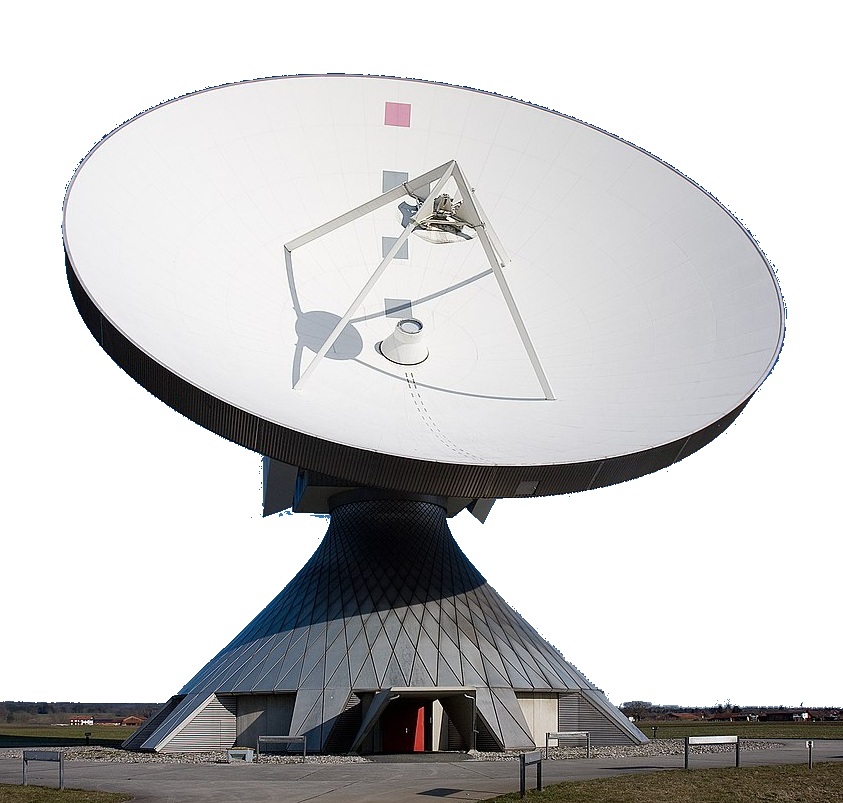
\includegraphics[width=0.7\linewidth]{dish.png}



Sometimes in a science museum, you will see two parabolic dishes far
apart and pointed at each other.  One person speaks with their mouth
at the focus of one.  The other person listens with their ear at the
focus of the other. Even though you are very far apart, it sounds like
they are really, really close.

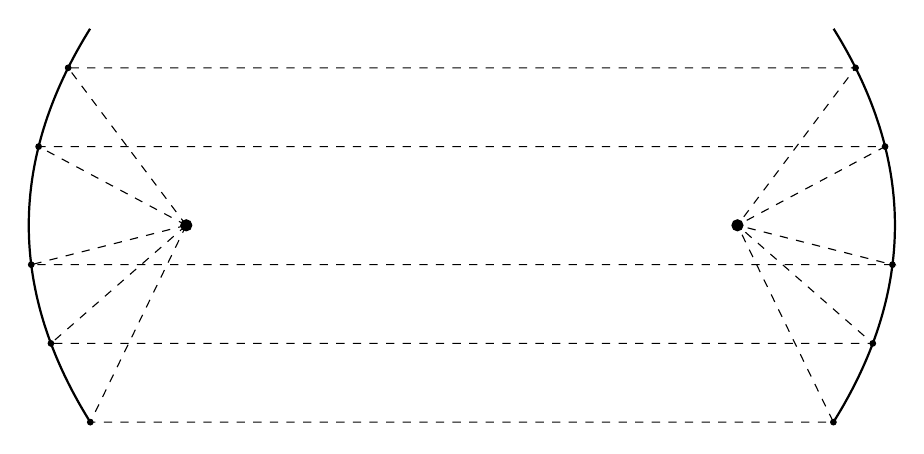
\begin{tikzpicture}
  \coordinate (f1) at (9, 0);
  \coordinate (f2) at (2, 0);
  \coordinate (p1) at (0.125, 1);
  \coordinate (p1d) at (10.875,1);
  \coordinate (p2) at (0.28125,-1.5);
  \coordinate (p2d) at (10.71875, -1.5);
  \coordinate (p3) at (0.5,2);
  \coordinate (p3d) at (10.5, 2);
  \coordinate (p4) at (0.03125, -0.5);
  \coordinate (p4d) at (10.96875, -0.5);
  \coordinate (p5) at (0.78125, -2.5);
  \coordinate (p5d) at (10.21875, -2.5);
  \draw[domain=-2.5:2.5,samples=300,variable=\x, thick]  plot ({0.125*\x*\x},\x);
  \draw[domain=-2.5:2.5,samples=300,variable=\x, thick]  plot ({11 - 0.125*\x*\x},\x);
  \filldraw  (f1) circle (2pt);
  \filldraw  (f2) circle (2pt);
  \filldraw  (p1) circle (1pt);
  \filldraw  (p1d) circle (1pt);
  \draw [thin,dashed] (f2) -- (p1) -- (p1d) -- (f1);
  \filldraw  (p2) circle (1pt);
  \filldraw  (p2d) circle (1pt);
  \draw [thin,dashed] (f2) -- (p2) -- (p2d) -- (f1);
  \filldraw  (p3) circle (1pt);
  \filldraw  (p3d) circle (1pt);
  \draw [thin,dashed] (f2) -- (p3) -- (p3d)--(f1);
  \filldraw  (p4) circle (1pt);
  \filldraw  (p4d) circle (1pt);
  \draw [thin,dashed] (f2) -- (p4) -- (p4d) -- (f1);
  \filldraw  (p5) circle (1pt);
  \filldraw  (p5d) circle (1pt);
  \draw [thin,dashed] (f2) -- (p5) -- (p5d) -- (f1);
\end{tikzpicture}

This is because the speaker's parabolic wall focuses the sound energy
in a nice beam the size of the wall pointed straight at the listener's
parabolic wall.  The listener's wall focuses the energy of that beam
at the listener's ear.

